


\documentclass[conference]{IEEEtran}
% Some Computer Society conferences also require the compsoc mode option,
% but others use the standard conference format.
%
% If IEEEtran.cls has not been installed into the LaTeX system files,
% manually specify the path to it like:
% \documentclass[conference]{../sty/IEEEtran}





% Some very useful LaTeX packages include:
% (uncomment the ones you want to load)


% *** MISC UTILITY PACKAGES ***
%
%\usepackage{ifpdf}
% Heiko Oberdiek's ifpdf.sty is very useful if you need conditional
% compilation based on whether the output is pdf or dvi.
% usage:
% \ifpdf
%   % pdf code
% \else
%   % dvi code
% \fi
% The latest version of ifpdf.sty can be obtained from:
% http://www.ctan.org/pkg/ifpdf
% Also, note that IEEEtran.cls V1.7 and later provides a builtin
% \ifCLASSINFOpdf conditional that works the same way.
% When switching from latex to pdflatex and vice-versa, the compiler may
% have to be run twice to clear warning/error messages.






% *** CITATION PACKAGES ***
%
\usepackage{cite}
% cite.sty was written by Donald Arseneau
% V1.6 and later of IEEEtran pre-defines the format of the cite.sty package
% \cite{} output to follow that of the IEEE. Loading the cite package will
% result in citation numbers being automatically sorted and properly
% "compressed/ranged". e.g., [1], [9], [2], [7], [5], [6] without using
% cite.sty will become [1], [2], [5]--[7], [9] using cite.sty. cite.sty's
% \cite will automatically add leading space, if needed. Use cite.sty's
% noadjust option (cite.sty V3.8 and later) if you want to turn this off
% such as if a citation ever needs to be enclosed in parenthesis.
% cite.sty is already installed on most LaTeX systems. Be sure and use
% version 5.0 (2009-03-20) and later if using hyperref.sty.
% The latest version can be obtained at:
% http://www.ctan.org/pkg/cite
% The documentation is contained in the cite.sty file itself.






% *** GRAPHICS RELATED PACKAGES ***
%
\ifCLASSINFOpdf
  % \usepackage[pdftex]{graphicx}
  % declare the path(s) where your graphic files are
  % \graphicspath{{../pdf/}{../jpeg/}}
  % and their extensions so you won't have to specify these with
  % every instance of \includegraphics
  % \DeclareGraphicsExtensions{.pdf,.jpeg,.png}
\else
  % or other class option (dvipsone, dvipdf, if not using dvips). graphicx
  % will default to the driver specified in the system graphics.cfg if no
  % driver is specified.
  % \usepackage[dvips]{graphicx}
  % declare the path(s) where your graphic files are
  % \graphicspath{{../eps/}}
  % and their extensions so you won't have to specify these with
  % every instance of \includegraphics
  % \DeclareGraphicsExtensions{.eps}
\fi
% graphicx was written by David Carlisle and Sebastian Rahtz. It is
% required if you want graphics, photos, etc. graphicx.sty is already
% installed on most LaTeX systems. The latest version and documentation
% can be obtained at: 
% http://www.ctan.org/pkg/graphicx
% Another good source of documentation is "Using Imported Graphics in
% LaTeX2e" by Keith Reckdahl which can be found at:
% http://www.ctan.org/pkg/epslatex
%
% latex, and pdflatex in dvi mode, support graphics in encapsulated
% postscript (.eps) format. pdflatex in pdf mode supports graphics
% in .pdf, .jpeg, .png and .mps (metapost) formats. Users should ensure
% that all non-photo figures use a vector format (.eps, .pdf, .mps) and
% not a bitmapped formats (.jpeg, .png). The IEEE frowns on bitmapped formats
% which can result in "jaggedy"/blurry rendering of lines and letters as
% well as large increases in file sizes.
%
% You can find documentation about the pdfTeX application at:
% http://www.tug.org/applications/pdftex





% *** MATH PACKAGES ***
%
\usepackage{amsmath}
% A popular package from the American Mathematical Society that provides
% many useful and powerful commands for dealing with mathematics.
%
% Note that the amsmath package sets \interdisplaylinepenalty to 10000
% thus preventing page breaks from occurring within multiline equations. Use:
%\interdisplaylinepenalty=2500
% after loading amsmath to restore such page breaks as IEEEtran.cls normally
% does. amsmath.sty is already installed on most LaTeX systems. The latest
% version and documentation can be obtained at:
% http://www.ctan.org/pkg/amsmath





% *** SPECIALIZED LIST PACKAGES ***
%
%\usepackage{algorithmic}
% algorithmic.sty was written by Peter Williams and Rogerio Brito.
% This package provides an algorithmic environment fo describing algorithms.
% You can use the algorithmic environment in-text or within a figure
% environment to provide for a floating algorithm. Do NOT use the algorithm
% floating environment provided by algorithm.sty (by the same authors) or
% algorithm2e.sty (by Christophe Fiorio) as the IEEE does not use dedicated
% algorithm float types and packages that provide these will not provide
% correct IEEE style captions. The latest version and documentation of
% algorithmic.sty can be obtained at:
% http://www.ctan.org/pkg/algorithms
% Also of interest may be the (relatively newer and more customizable)
% algorithmicx.sty package by Szasz Janos:
% http://www.ctan.org/pkg/algorithmicx




% *** ALIGNMENT PACKAGES ***
%
\usepackage{array}
% Frank Mittelbach's and David Carlisle's array.sty patches and improves
% the standard LaTeX2e array and tabular environments to provide better
% appearance and additional user controls. As the default LaTeX2e table
% generation code is lacking to the point of almost being broken with
% respect to the quality of the end results, all users are strongly
% advised to use an enhanced (at the very least that provided by array.sty)
% set of table tools. array.sty is already installed on most systems. The
% latest version and documentation can be obtained at:
% http://www.ctan.org/pkg/array


% IEEEtran contains the IEEEeqnarray family of commands that can be used to
% generate multiline equations as well as matrices, tables, etc., of high
% quality.




% *** SUBFIGURE PACKAGES ***
%\ifCLASSOPTIONcompsoc
%  \usepackage[caption=false,font=normalsize,labelfont=sf,textfont=sf]{subfig}
%\else
%  \usepackage[caption=false,font=footnotesize]{subfig}
%\fi
% subfig.sty, written by Steven Douglas Cochran, is the modern replacement
% for subfigure.sty, the latter of which is no longer maintained and is
% incompatible with some LaTeX packages including fixltx2e. However,
% subfig.sty requires and automatically loads Axel Sommerfeldt's caption.sty
% which will override IEEEtran.cls' handling of captions and this will result
% in non-IEEE style figure/table captions. To prevent this problem, be sure
% and invoke subfig.sty's "caption=false" package option (available since
% subfig.sty version 1.3, 2005/06/28) as this is will preserve IEEEtran.cls
% handling of captions.
% Note that the Computer Society format requires a larger sans serif font
% than the serif footnote size font used in traditional IEEE formatting
% and thus the need to invoke different subfig.sty package options depending
% on whether compsoc mode has been enabled.
%
% The latest version and documentation of subfig.sty can be obtained at:
% http://www.ctan.org/pkg/subfig




% *** FLOAT PACKAGES ***
%
%\usepackage{fixltx2e}
% fixltx2e, the successor to the earlier fix2col.sty, was written by
% Frank Mittelbach and David Carlisle. This package corrects a few problems
% in the LaTeX2e kernel, the most notable of which is that in current
% LaTeX2e releases, the ordering of single and double column floats is not
% guaranteed to be preserved. Thus, an unpatched LaTeX2e can allow a
% single column figure to be placed prior to an earlier double column
% figure.
% Be aware that LaTeX2e kernels dated 2015 and later have fixltx2e.sty's
% corrections already built into the system in which case a warning will
% be issued if an attempt is made to load fixltx2e.sty as it is no longer
% needed.
% The latest version and documentation can be found at:
% http://www.ctan.org/pkg/fixltx2e


%\usepackage{stfloats}
% stfloats.sty was written by Sigitas Tolusis. This package gives LaTeX2e
% the ability to do double column floats at the bottom of the page as well
% as the top. (e.g., "\begin{figure*}[!b]" is not normally possible in
% LaTeX2e). It also provides a command:
%\fnbelowfloat
% to enable the placement of footnotes below bottom floats (the standard
% LaTeX2e kernel puts them above bottom floats). This is an invasive package
% which rewrites many portions of the LaTeX2e float routines. It may not work
% with other packages that modify the LaTeX2e float routines. The latest
% version and documentation can be obtained at:
% http://www.ctan.org/pkg/stfloats
% Do not use the stfloats baselinefloat ability as the IEEE does not allow
% \baselineskip to stretch. Authors submitting work to the IEEE should note
% that the IEEE rarely uses double column equations and that authors should try
% to avoid such use. Do not be tempted to use the cuted.sty or midfloat.sty
% packages (also by Sigitas Tolusis) as the IEEE does not format its papers in
% such ways.
% Do not attempt to use stfloats with fixltx2e as they are incompatible.
% Instead, use Morten Hogholm'a dblfloatfix which combines the features
% of both fixltx2e and stfloats:
%
% \usepackage{dblfloatfix}
% The latest version can be found at:
% http://www.ctan.org/pkg/dblfloatfix




% *** PDF, URL AND HYPERLINK PACKAGES ***
%
%\usepackage{url}
% url.sty was written by Donald Arseneau. It provides better support for
% handling and breaking URLs. url.sty is already installed on most LaTeX
% systems. The latest version and documentation can be obtained at:
% http://www.ctan.org/pkg/url
% Basically, \url{my_url_here}.





% *** Do not adjust lengths that control margins, column widths, etc. ***
% *** Do not use packages that alter fonts (such as pslatex).         ***
% There should be no need to do such things with IEEEtran.cls V1.6 and later.
% (Unless specifically asked to do so by the journal or conference you plan
% to submit to, of course. )


% correct bad hyphenation here
\hyphenation{op-tical net-works semi-conduc-tor}


\usepackage{tikz}
\usetikzlibrary{shapes,arrows,positioning}
\usepackage{pgfplots}
\pgfplotsset{compat=1.7}
\usepackage{pgfplotstable}
\pgfplotstableset{col sep=comma}
\newcommand{\APW}{\ensuremath{w_A}}
\newcommand{\VPW}{\ensuremath{w_V}}
\newcommand{\APH}{\ensuremath{h_A}}
\newcommand{\VPH}{\ensuremath{h_V}}
\DeclareMathOperator{\sgn}{sign}
\DeclareMathOperator*{\argmin}{arg\,min}

\begin{document}
%
% paper title
% Titles are generally capitalized except for words such as a, an, and, as,
% at, but, by, for, in, nor, of, on, or, the, to and up, which are usually
% not capitalized unless they are the first or last word of the title.
% Linebreaks \\ can be used within to get better formatting as desired.
% Do not put math or special symbols in the title.
\title{Real-Time, Data-Driven System to Learn
Parameters for Multisite Pacemaker Beat Detection}


% author names and affiliations
% use a multiple column layout for up to three different
% affiliations
\author{\IEEEauthorblockN{Yamin Arefeen\IEEEauthorrefmark{1}, Philip Taffet\IEEEauthorrefmark{2}, Daniel Zdeblick\IEEEauthorrefmark{1}, Jorge Quintero\IEEEauthorrefmark{1}, Greg Harper\IEEEauthorrefmark{1},\\
Behnaam Aazhang\IEEEauthorrefmark{1}, Joseph Cavallaro\IEEEauthorrefmark{1}, and Mehdi Razavi\IEEEauthorrefmark{3}}
\IEEEauthorblockA{\IEEEauthorrefmark{1}Department of Electrical and Computer Engineering, \IEEEauthorrefmark{2}Department of Computer Science\\
	Rice University, Houston, TX}
	\IEEEauthorblockA{\IEEEauthorrefmark{3}Department of Cardiology\\
Texas Heart Institute, Houston, TX}
	\IEEEauthorblockA{yarefeen@mit.edu, zdeblick@uw.edu, ptaffet@rice.edu, aaz@rice.edu, cavallar@rice.edu, razavi@bcm.edu}
}

% conference papers do not typically use \thanks and this command
% is locked out in conference mode. If really needed, such as for
% the acknowledgment of grants, issue a \IEEEoverridecommandlockouts
% after \documentclass


% use for special paper notices
%\IEEEspecialpapernotice{(Invited Paper)}




% make the title area
\maketitle

% As a general rule, do not put math, special symbols or citations
% in the abstract
% no keywords




% For peer review papers, you can put extra information on the cover
% page as needed:
% \ifCLASSOPTIONpeerreview
% \begin{center} \bfseries EDICS Category: 3-BBND \end{center}
% \fi
%
% For peerreview papers, this IEEEtran command inserts a page break and
% creates the second title. It will be ignored for other modes.

Cardiac diseases are the most common cause of death in the United States. 
More than 600,000 people die each year due to some form of heart disease. 
To combat heart failure, doctors implant artificial electronic pacemakers that stimulate the heart to contract artificially through externally supplied electrical pulses. 
 Current pacemakers use the DDDR algorithm to determine whether the heart requires stimulation from a cardiac electrical signal. 
 Doctors must manually specify parameters in the algorithm for each individual patient in order to tune the detection algorithm to the patient�s physiology. 
 Additionally, current pacemakers are often unable to distinguish between atrial and ventricular beats. 
Our paper serves as the first iteration of a multiple year long research project that aims to combat this issue by designing
a pacemaker that utilizes multiple wireless sensors on the heart to both sense and stimulate with unprecedented resolution.
\figurename~\ref{fig:wireless} showcases the ultimate vision of the multiyear research project.
In addition, accurate distinction between the two portions allows for a more effective form of pacing known as Cardiac Resynchronization Therapy (CRT). 
However, 30\% of patients with pacemakers do not respond to CRT implemented by current pacemakers.
\begin{figure}[h]
	\centering
	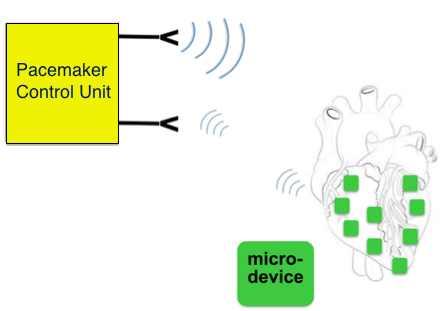
\includegraphics[width=.8\columnwidth]{wireless.png}
	\caption{Wireless micro-devices sensing the heart and communicating with the control unit that will house our algorithm.  Our algorithm will learn beat detection parameters for each wireless micro device.}
	\label{fig:wireless}
\end{figure}

To efficiently learn parameters for the multiple wireless sensors and make beat detection more suitable for CRT, we propose a learning algorithm that learns the height of an atrial peak (\APH{}), the height of a ventricular peak (\VPH{}), the width of an atrial peak (\APW{}), and the width of a ventricular peak (\VPW{}) within a signal by simply processing 10 seconds of data sampled at 1 kHz (see \figurename~\ref{fig:singlebeat}). 
We use these parameters in atrial and ventricular beat detection to illustrate that our learned parameters can be used to distinguish between atrial and ventricular beats in a signal. 
Additionally, we implement the algorithm on a Field Programmable Gate Array to demonstrate that the algorithm can be run on a real-time system.
\begin{figure}
	\centering
	\begin{tikzpicture}
		\begin{axis}[
				%title      =,
				xlabel     = Time (ms),
				ylabel     = Voltage (mV),
				legend pos = south west,
			]
			\addplot+[mark=none,smooth, black] table[x = t, y = v, col sep=comma]{singlebeat.csv} ;
			% \draw[densely dotted] (axis cs:78, 796) -- (axis cs:95, 461) ;
			\draw[red] (axis cs:78, 1100) -- ++(0, 2pt) -- ++(0, -4pt) -- ++(0, 2pt) -- (axis cs:95, 1100) node(m1) [midway] {} -- ++(0, 2pt) -- ++(0, -4pt);
			\draw[red] (axis cs:50, 590) -- ++(2pt, 0) -- ++(-4pt, 0) -- ++(2pt, 0) -- (axis cs: 50, 0) node(m2) [midway] {} -- ++(2pt, 0) -- ++(-4pt, 0) ;
			\node[pin=75:{\APW}] at (m1) {};
			\node[pin={[pin distance=8pt]120:{\APH}}] at (m2) {};
			% \draw (axis cs:78, 580) -- (axis cs:78, 680) -- (axis cs: 78, 630) -- (axis cs:95, 630) -- (axis cs:95, 580) -- (axis cs:95, 680);

			\draw[blue] (axis cs:408, 2000) -- ++(0, 2pt) -- ++(0, -4pt) -- ++(0, 2pt) -- (axis cs:416, 2000) node(m3)[midway] {} -- ++(0, 2pt) -- ++(0, -4pt);
			%\draw[densely dotted] (axis cs:408, 1460) -- (axis cs:416, 1085) ;
			%\draw (axis cs:408, 1220) -- (axis cs:408, 1320) -- (axis cs: 408, 1270) -- (axis cs:416, 1270) -- (axis cs:416, 1220) -- (axis cs:416, 1320);


			\draw[blue] (axis cs:430, 1160) -- ++(2pt, 0) -- ++(-4pt, 0) -- ++(2pt, 0) -- (axis cs: 430, 0) node(m4)[midway] {} -- ++(2pt, 0) -- ++(-4pt, 0) ;
			\node[pin={[pin distance=8pt]200:{\VPW}}] at (m3) {};
			\node[pin={[pin distance=3pt]350:{\VPH}}] at (m4) {};
			\legend{$f[n]$}
		\end{axis}
	\end{tikzpicture}
	\caption{
	A segment of CES containing a single atrial and ventricular beat, labeled with the parameters \APH, \VPH, \APW, and \VPW. 
	Notice that the atrial beat is wider but smaller than the ventricular beat.}
	\label{fig:singlebeat}
\end{figure}

Our algorithm begins by learning \APW{} and \VPW{} on 10 seconds of cardiac electrical data. 
In order to learn the two width parameters for peak detection, our system uses a nonparametric algorithm that finds and extracts features of all peak-shaped patterns in the training waveform that could correspond to beats. 
It then uses k-means, with k = 2, to segregate the patterns into ones that correspond to ventricular beats and those that correspond to atrial beats, and then extracts the lengths from the centers of each cluster. 


After learning \VPW{} and \APW{}, we proceed on the same segment of cardiac electrical signal to learn \VPH{} and \APH{}. 
The basic strategy of the peak height threshold learning is to look for a large range of thresholds that detects the same number of ventricular beats in the cardiac electrical signal. 
This idea follows from the observation that there is typically a wide range of thresholds that are high enough to exclude the lower (typically atrial) beats but low enough to detect each of the higher (typically ventricular) beats. 
As the algorithm tries thresholds lower than that range, it starts to detect lower beats, and as it tries thresholds higher than that range, it stops detecting some of the higher beats, so the number of detected beats begins to change. 

The height threshold learning algorithm is effectively a search algorithm for the longest and flattest interval of the function $\beta(\tau)$, which we define as follows.
\begin{multline*}
	\beta(\tau) = \\\text{Number of beats detected in } f[n] \text{ using } \tau \text{ as a threshold}
\end{multline*}
\begin{figure}
	\centering
	\begin{tikzpicture}
		\begin{axis}[
				title      = $\beta(\tau)$,
				xlabel     = Threshold (mV),
				ylabel     = Number of beats,
				legend pos = north east,
				restrict y to domain* = 0:300
			]
			\addplot+[mark=none] table[x = th, y = beats, col sep=comma]{beats.csv} ;
		\end{axis}
	\end{tikzpicture}
	\caption{Graph of the function $\beta(\tau)$ on example CES data. The long flat segments correspond to potentially good threshold choices.}
	\label{fig:beats}
\end{figure}
However, computing $\beta(\tau)$ for even a single value of $\tau$ is somewhat computationally expensive, so we try to minimize the number of thresholds for which we compute it.
Our algorithm uses bounded recursive refinement, and it essentially samples the function $\beta(\tau)$. 
We call this the ``Flat-Finding'' algorithm for ventricular and atrial heights. 
 An extensive description of both of our algorithms can be found in the complete paper.

In the future, we envision that our algorithm will be implemented in real pacemakers. 
In order to demonstrate that our proposed solution can run in real-time on hardware that can be shrunk down to the size of an integrated circuit, we fully implemented our algorithm on a Field Programmable Gate Array (FPGA). 
In addition, to test on analog signals, we designed an analog preprocessing circuit board that filters and cleans the signal from the heart before it is digitized and processed by the algorithm running on the FPGA.

To validate our solution, we implemented our algorithms in
Matlab and performed atrial and ventricular beat
detection using learned parameters on
data provided by colleagues at the Texas Heart Institute.
In order to record the data, an in vivo,
live animal study procedure was performed. For a single
animal, 17 bipolar electrodes were placed on the left ventricle
of the heart. Each electrode sensed electrical activity
directly from the heart for one minute and digitized the
signal at a 1 kHz sampling rate.
This was done for 3 animals, giving us a total
of 51 channels, where each channel is one minute of cardiac electrical signal.

Our detection error rates are sufficiently low across all 51 channels (see Table~\ref{tab:errors}). 
 Since we performed atrial and ventricular beat detection based on the parameters that our algorithm learned, the algorithm clearly learned \APW{}, \VPW{}, \APH{}, and \VPH{} correctly for the vast majority of channels. 

\begin{table}[h]
	\caption{Detection Error Rates using Learned Parameters}
	\label{tab:errors}
	\centering
	\begin{tabular}{|c|c|c|}
		\hline
		Type & False Positive Error Rate & False Negative Error Rate \\
		\hline 
		Ventricles & 0.16\% &4.77\% \\
		\hline
		Atria & 0.89\% & 4.59\% \\
		\hline
		Total & 0.50\% & 4.70 \% \\
		\hline
	\end{tabular}
\end{table}
In order to validate the hardware implementation of our algorithm, we interfaced our system to a Langendorff heart. 
We connected our preprocessor to ordinary wires sutured to the Langendroff heart, and then used our FPGA to run our algorithm on the cardiac signal. 
Our system correctly sensed signals using the preprocessor, learned pacing parameters (\VPW{} and \VPH{}), and detected ventricular beats using the learned values of \VPW{} and \VPH{} in real time.

We have demonstrated a working algorithm implemented on hardware that correctly learns \APH{}, \VPH{}, \APW{}, and \VPW{}. 
Additionally, these parameters can be reliably used to distinguish between atrial and ventricular beats in a cardiac electrical signal in real time. 




% An example of a floating figure using the graphicx package.
% Note that \label must occur AFTER (or within) \caption.
% For figures, \caption should occur after the \includegraphics.
% Note that IEEEtran v1.7 and later has special internal code that
% is designed to preserve the operation of \label within \caption
% even when the captionsoff option is in effect. However, because
% of issues like this, it may be the safest practice to put all your
% \label just after \caption rather than within \caption{}.
%
% Reminder: the "draftcls" or "draftclsnofoot", not "draft", class
% option should be used if it is desired that the figures are to be
% displayed while in draft mode.
%
%\begin{figure}[!t]
%\centering
%\includegraphics[width=2.5in]{myfigure}
% where an .eps filename suffix will be assumed under latex, 
% and a .pdf suffix will be assumed for pdflatex; or what has been declared
% via \DeclareGraphicsExtensions.
%\caption{Simulation results for the network.}
%\label{fig_sim}
%\end{figure}

% Note that the IEEE typically puts floats only at the top, even when this
% results in a large percentage of a column being occupied by floats.


% An example of a double column floating figure using two subfigures.
% (The subfig.sty package must be loaded for this to work.)
% The subfigure \label commands are set within each subfloat command,
% and the \label for the overall figure must come after \caption.
% \hfil is used as a separator to get equal spacing.
% Watch out that the combined width of all the subfigures on a 
% line do not exceed the text width or a line break will occur.
%
%\begin{figure*}[!t]
%\centering
%\subfloat[Case I]{\includegraphics[width=2.5in]{box}%
%\label{fig_first_case}}
%\hfil
%\subfloat[Case II]{\includegraphics[width=2.5in]{box}%
%\label{fig_second_case}}
%\caption{Simulation results for the network.}
%\label{fig_sim}
%\end{figure*}
%
% Note that often IEEE papers with subfigures do not employ subfigure
% captions (using the optional argument to \subfloat[]), but instead will
% reference/describe all of them (a), (b), etc., within the main caption.
% Be aware that for subfig.sty to generate the (a), (b), etc., subfigure
% labels, the optional argument to \subfloat must be present. If a
% subcaption is not desired, just leave its contents blank,
% e.g., \subfloat[].


% An example of a floating table. Note that, for IEEE style tables, the
% \caption command should come BEFORE the table and, given that table
% captions serve much like titles, are usually capitalized except for words
% such as a, an, and, as, at, but, by, for, in, nor, of, on, or, the, to
% and up, which are usually not capitalized unless they are the first or
% last word of the caption. Table text will default to \footnotesize as
% the IEEE normally uses this smaller font for tables.
% The \label must come after \caption as always.
%
%\begin{table}[!t]
%% increase table row spacing, adjust to taste
%\renewcommand{\arraystretch}{1.3}
% if using array.sty, it might be a good idea to tweak the value of
% \extrarowheight as needed to properly center the text within the cells
%\caption{An Example of a Table}
%\label{table_example}
%\centering
%% Some packages, such as MDW tools, offer better commands for making tables
%% than the plain LaTeX2e tabular which is used here.
%\begin{tabular}{|c||c|}
%\hline
%One & Two\\
%\hline
%Three & Four\\
%\hline
%\end{tabular}
%\end{table}


% Note that the IEEE does not put floats in the very first column
% - or typically anywhere on the first page for that matter. Also,
% in-text middle ("here") positioning is typically not used, but it
% is allowed and encouraged for Computer Society conferences (but
% not Computer Society journals). Most IEEE journals/conferences use
% top floats exclusively. 
% Note that, LaTeX2e, unlike IEEE journals/conferences, places
% footnotes above bottom floats. This can be corrected via the
% \fnbelowfloat command of the stfloats package.




% trigger a \newpage just before the given reference
% number - used to balance the columns on the last page
% adjust value as needed - may need to be readjusted if
% the document is modified later
%\IEEEtriggeratref{8}
% The "triggered" command can be changed if desired:
%\IEEEtriggercmd{\enlargethispage{-5in}}

% references section

% can use a bibliography generated by BibTeX as a .bbl file
% BibTeX documentation can be easily obtained at:
% http://mirror.ctan.org/biblio/bibtex/contrib/doc/
% The IEEEtran BibTeX style support page is at:
% http://www.michaelshell.org/tex/ieeetran/bibtex/
% argument is your BibTeX string definitions and bibliography database(s)



% that's all folks
\end{document}


